\documentclass[twoside]{book}

% Packages required by doxygen
\usepackage{fixltx2e}
\usepackage{calc}
\usepackage{doxygen}
\usepackage[export]{adjustbox} % also loads graphicx
\usepackage{graphicx}
\usepackage[utf8]{inputenc}
\usepackage{makeidx}
\usepackage{multicol}
\usepackage{multirow}
\PassOptionsToPackage{warn}{textcomp}
\usepackage{textcomp}
\usepackage[nointegrals]{wasysym}
\usepackage[table]{xcolor}

% Font selection
\usepackage[T1]{fontenc}
\usepackage[scaled=.90]{helvet}
\usepackage{courier}
\usepackage{amssymb}
\usepackage{sectsty}
\renewcommand{\familydefault}{\sfdefault}
\allsectionsfont{%
  \fontseries{bc}\selectfont%
  \color{darkgray}%
}
\renewcommand{\DoxyLabelFont}{%
  \fontseries{bc}\selectfont%
  \color{darkgray}%
}
\newcommand{\+}{\discretionary{\mbox{\scriptsize$\hookleftarrow$}}{}{}}

% Page & text layout
\usepackage{geometry}
\geometry{%
  a4paper,%
  top=2.5cm,%
  bottom=2.5cm,%
  left=2.5cm,%
  right=2.5cm%
}
\tolerance=750
\hfuzz=15pt
\hbadness=750
\setlength{\emergencystretch}{15pt}
\setlength{\parindent}{0cm}
\setlength{\parskip}{3ex plus 2ex minus 2ex}
\makeatletter
\renewcommand{\paragraph}{%
  \@startsection{paragraph}{4}{0ex}{-1.0ex}{1.0ex}{%
    \normalfont\normalsize\bfseries\SS@parafont%
  }%
}
\renewcommand{\subparagraph}{%
  \@startsection{subparagraph}{5}{0ex}{-1.0ex}{1.0ex}{%
    \normalfont\normalsize\bfseries\SS@subparafont%
  }%
}
\makeatother

% Headers & footers
\usepackage{fancyhdr}
\pagestyle{fancyplain}
\fancyhead[LE]{\fancyplain{}{\bfseries\thepage}}
\fancyhead[CE]{\fancyplain{}{}}
\fancyhead[RE]{\fancyplain{}{\bfseries\leftmark}}
\fancyhead[LO]{\fancyplain{}{\bfseries\rightmark}}
\fancyhead[CO]{\fancyplain{}{}}
\fancyhead[RO]{\fancyplain{}{\bfseries\thepage}}
\fancyfoot[LE]{\fancyplain{}{}}
\fancyfoot[CE]{\fancyplain{}{}}
\fancyfoot[RE]{\fancyplain{}{\bfseries\scriptsize Generated by Doxygen }}
\fancyfoot[LO]{\fancyplain{}{\bfseries\scriptsize Generated by Doxygen }}
\fancyfoot[CO]{\fancyplain{}{}}
\fancyfoot[RO]{\fancyplain{}{}}
\renewcommand{\footrulewidth}{0.4pt}
\renewcommand{\chaptermark}[1]{%
  \markboth{#1}{}%
}
\renewcommand{\sectionmark}[1]{%
  \markright{\thesection\ #1}%
}

% Indices & bibliography
\usepackage{natbib}
\usepackage[titles]{tocloft}
\setcounter{tocdepth}{3}
\setcounter{secnumdepth}{5}
\makeindex

% Hyperlinks (required, but should be loaded last)
\usepackage{ifpdf}
\ifpdf
  \usepackage[pdftex,pagebackref=true]{hyperref}
\else
  \usepackage[ps2pdf,pagebackref=true]{hyperref}
\fi
\hypersetup{%
  colorlinks=true,%
  linkcolor=blue,%
  citecolor=blue,%
  unicode%
}

% Custom commands
\newcommand{\clearemptydoublepage}{%
  \newpage{\pagestyle{empty}\cleardoublepage}%
}

\usepackage{caption}
\captionsetup{labelsep=space,justification=centering,font={bf},singlelinecheck=off,skip=4pt,position=top}

%===== C O N T E N T S =====

\begin{document}

% Titlepage & ToC
\hypersetup{pageanchor=false,
             bookmarksnumbered=true,
             pdfencoding=unicode
            }
\pagenumbering{alph}
\begin{titlepage}
\vspace*{7cm}
\begin{center}%
{\Large My Project }\\
\vspace*{1cm}
{\large Generated by Doxygen 1.8.13}\\
\end{center}
\end{titlepage}
\clearemptydoublepage
\pagenumbering{roman}
\tableofcontents
\clearemptydoublepage
\pagenumbering{arabic}
\hypersetup{pageanchor=true}

%--- Begin generated contents ---
\chapter{binary\+Clock}
\label{md_README}
\Hypertarget{md_README}
\input{md_README}
\chapter{Class Index}
\section{Class List}
Here are the classes, structs, unions and interfaces with brief descriptions\+:\begin{DoxyCompactList}
\item\contentsline{section}{\hyperlink{classBCD}{B\+CD} }{\pageref{classBCD}}{}
\item\contentsline{section}{\hyperlink{classbin__Clock}{bin\+\_\+\+Clock} }{\pageref{classbin__Clock}}{}
\end{DoxyCompactList}

\chapter{Class Documentation}
\hypertarget{classBCD}{}\section{B\+CD Class Reference}
\label{classBCD}\index{B\+CD@{B\+CD}}
\subsection*{Public Member Functions}
\begin{DoxyCompactItemize}
\item 
\hyperlink{classBCD_a83b94116c047169535e9e61aab6d6bb3}{B\+CD} (int decimal)
\begin{DoxyCompactList}\small\item\em Es el constructor del objeto \hyperlink{classBCD}{B\+CD} con parametros inicializa el número binario con el decimal asignado. \end{DoxyCompactList}\item 
\mbox{\Hypertarget{classBCD_a3d44b73ea05ac6ff8fe78ca08a1e78e6}\label{classBCD_a3d44b73ea05ac6ff8fe78ca08a1e78e6}} 
\hyperlink{classBCD_a3d44b73ea05ac6ff8fe78ca08a1e78e6}{B\+CD} ()
\begin{DoxyCompactList}\small\item\em Es el constructor del objeto \hyperlink{classBCD}{B\+CD} sin parametros inicializa el número binario en 0 y crea el arreglo que guardara al binario. \end{DoxyCompactList}\item 
void \hyperlink{classBCD_ae6596927da1233e50f527192f7171269}{set\+B\+CD} (int decimal)
\begin{DoxyCompactList}\small\item\em le asigna al objeto \hyperlink{classBCD}{B\+CD} el número decimal asignado. \end{DoxyCompactList}\item 
\mbox{\Hypertarget{classBCD_a7dc5f8bee9eca70567d6d5f09cc2c55f}\label{classBCD_a7dc5f8bee9eca70567d6d5f09cc2c55f}} 
void \hyperlink{classBCD_a7dc5f8bee9eca70567d6d5f09cc2c55f}{incrementar\+\_\+\+B\+CD} ()
\begin{DoxyCompactList}\small\item\em aumenta el valor del numero binario en 1 \end{DoxyCompactList}\item 
int \hyperlink{classBCD_a49603f54ebd9578939224cd5a5a8d96d}{get\+Suma} ()
\begin{DoxyCompactList}\small\item\em regresa el campo suma del objeto \hyperlink{classBCD}{B\+CD}. \end{DoxyCompactList}\end{DoxyCompactItemize}
\subsection*{Public Attributes}
\begin{DoxyCompactItemize}
\item 
\mbox{\Hypertarget{classBCD_aec89ba159a7db6c1f5542d94f56b257a}\label{classBCD_aec89ba159a7db6c1f5542d94f56b257a}} 
int {\bfseries suma}
\item 
\mbox{\Hypertarget{classBCD_ad8d6bae21dbf8ec970991ef5923b531c}\label{classBCD_ad8d6bae21dbf8ec970991ef5923b531c}} 
int $\ast$ {\bfseries bcd}
\end{DoxyCompactItemize}


\subsection{Constructor \& Destructor Documentation}
\mbox{\Hypertarget{classBCD_a83b94116c047169535e9e61aab6d6bb3}\label{classBCD_a83b94116c047169535e9e61aab6d6bb3}} 
\index{B\+CD@{B\+CD}!B\+CD@{B\+CD}}
\index{B\+CD@{B\+CD}!B\+CD@{B\+CD}}
\subsubsection{\texorpdfstring{B\+C\+D()}{BCD()}}
{\footnotesize\ttfamily B\+C\+D\+::\+B\+CD (\begin{DoxyParamCaption}\item[{int}]{decimal }\end{DoxyParamCaption})}



Es el constructor del objeto \hyperlink{classBCD}{B\+CD} con parametros inicializa el número binario con el decimal asignado. 


\begin{DoxyParams}{Parameters}
{\em decimal} & es el número decimal con el que se va a inicializar el número binario. \\
\hline
\end{DoxyParams}


\subsection{Member Function Documentation}
\mbox{\Hypertarget{classBCD_a49603f54ebd9578939224cd5a5a8d96d}\label{classBCD_a49603f54ebd9578939224cd5a5a8d96d}} 
\index{B\+CD@{B\+CD}!get\+Suma@{get\+Suma}}
\index{get\+Suma@{get\+Suma}!B\+CD@{B\+CD}}
\subsubsection{\texorpdfstring{get\+Suma()}{getSuma()}}
{\footnotesize\ttfamily int B\+C\+D\+::get\+Suma (\begin{DoxyParamCaption}{ }\end{DoxyParamCaption})}



regresa el campo suma del objeto \hyperlink{classBCD}{B\+CD}. 

\begin{DoxyReturn}{Returns}
suma es el campo suma del objeto que es el equivalente decimal al numero binario; 
\end{DoxyReturn}
\mbox{\Hypertarget{classBCD_ae6596927da1233e50f527192f7171269}\label{classBCD_ae6596927da1233e50f527192f7171269}} 
\index{B\+CD@{B\+CD}!set\+B\+CD@{set\+B\+CD}}
\index{set\+B\+CD@{set\+B\+CD}!B\+CD@{B\+CD}}
\subsubsection{\texorpdfstring{set\+B\+C\+D()}{setBCD()}}
{\footnotesize\ttfamily void B\+C\+D\+::set\+B\+CD (\begin{DoxyParamCaption}\item[{int}]{decimal }\end{DoxyParamCaption})}



le asigna al objeto \hyperlink{classBCD}{B\+CD} el número decimal asignado. 


\begin{DoxyParams}{Parameters}
{\em decimal} & es el número decimal que se le asiganrá al objeto \hyperlink{classBCD}{B\+CD}. \\
\hline
\end{DoxyParams}


The documentation for this class was generated from the following files\+:\begin{DoxyCompactItemize}
\item 
B\+C\+D.\+h\item 
B\+C\+D.\+cpp\end{DoxyCompactItemize}

\hypertarget{classbin__Clock}{}\section{bin\+\_\+\+Clock Class Reference}
\label{classbin__Clock}\index{bin\+\_\+\+Clock@{bin\+\_\+\+Clock}}


Collaboration diagram for bin\+\_\+\+Clock\+:
\nopagebreak
\begin{figure}[H]
\begin{center}
\leavevmode
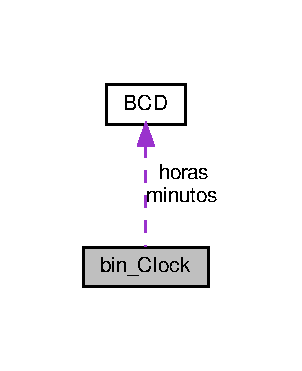
\includegraphics[width=145pt]{classbin__Clock__coll__graph}
\end{center}
\end{figure}
\subsection*{Public Member Functions}
\begin{DoxyCompactItemize}
\item 
\mbox{\Hypertarget{classbin__Clock_af4bb98f6018065cfda88fbc00d7c4c9c}\label{classbin__Clock_af4bb98f6018065cfda88fbc00d7c4c9c}} 
\hyperlink{classbin__Clock_af4bb98f6018065cfda88fbc00d7c4c9c}{bin\+\_\+\+Clock} ()
\begin{DoxyCompactList}\small\item\em Constructor que crea un reloj inicializado en 00\+:00\+:00. \end{DoxyCompactList}\item 
\hyperlink{classbin__Clock_a08180ca924ba3cf39b87fad8faafc5cc}{bin\+\_\+\+Clock} (int hora, int mins)
\begin{DoxyCompactList}\small\item\em Constructor que crea un reloj inicializado con los parametros que se le dan y los segundos en 00. \end{DoxyCompactList}\item 
\mbox{\Hypertarget{classbin__Clock_a3a6acf30477a05b6bb743d5b2317100b}\label{classbin__Clock_a3a6acf30477a05b6bb743d5b2317100b}} 
void \hyperlink{classbin__Clock_a3a6acf30477a05b6bb743d5b2317100b}{incrementar\+\_\+\+Clock} ()
\begin{DoxyCompactList}\small\item\em Metodo que incrementa en 1 los minutos del reloj. \end{DoxyCompactList}\item 
\mbox{\Hypertarget{classbin__Clock_ad8d8de67aa7e8b6e55ccc2a8e2cb64b1}\label{classbin__Clock_ad8d8de67aa7e8b6e55ccc2a8e2cb64b1}} 
void \hyperlink{classbin__Clock_ad8d8de67aa7e8b6e55ccc2a8e2cb64b1}{reset\+\_\+\+Clock} ()
\begin{DoxyCompactList}\small\item\em Metodo que reinicia el reloj a 00\+:00\+:00. \end{DoxyCompactList}\end{DoxyCompactItemize}
\subsection*{Public Attributes}
\begin{DoxyCompactItemize}
\item 
\mbox{\Hypertarget{classbin__Clock_ae38c8d386ad53284942a97e7002f0131}\label{classbin__Clock_ae38c8d386ad53284942a97e7002f0131}} 
\hyperlink{classBCD}{B\+CD} {\bfseries horas}
\item 
\mbox{\Hypertarget{classbin__Clock_a175417b7491035e0b201113d37ca55dc}\label{classbin__Clock_a175417b7491035e0b201113d37ca55dc}} 
\hyperlink{classBCD}{B\+CD} {\bfseries minutos}
\end{DoxyCompactItemize}


\subsection{Constructor \& Destructor Documentation}
\mbox{\Hypertarget{classbin__Clock_a08180ca924ba3cf39b87fad8faafc5cc}\label{classbin__Clock_a08180ca924ba3cf39b87fad8faafc5cc}} 
\index{bin\+\_\+\+Clock@{bin\+\_\+\+Clock}!bin\+\_\+\+Clock@{bin\+\_\+\+Clock}}
\index{bin\+\_\+\+Clock@{bin\+\_\+\+Clock}!bin\+\_\+\+Clock@{bin\+\_\+\+Clock}}
\subsubsection{\texorpdfstring{bin\+\_\+\+Clock()}{bin\_Clock()}}
{\footnotesize\ttfamily bin\+\_\+\+Clock\+::bin\+\_\+\+Clock (\begin{DoxyParamCaption}\item[{int}]{hora,  }\item[{int}]{mins }\end{DoxyParamCaption})}



Constructor que crea un reloj inicializado con los parametros que se le dan y los segundos en 00. 


\begin{DoxyParams}{Parameters}
{\em hora} & Entero que indica la hora con la que se inicializara el reloj. \\
\hline
{\em mins} & Entero que indica los minutos con los que se inicializara el reloj. \\
\hline
\end{DoxyParams}


The documentation for this class was generated from the following files\+:\begin{DoxyCompactItemize}
\item 
bin\+Clock.\+h\item 
bin\+Clock.\+cpp\end{DoxyCompactItemize}

%--- End generated contents ---

% Index
\backmatter
\newpage
\phantomsection
\clearemptydoublepage
\addcontentsline{toc}{chapter}{Index}
\printindex

\end{document}
